% !TeX spellcheck = nl_NL
\documentclass{article}

\begin{document}
	\subsection{Een Cassandra cluster opzetten}
	Nu we onze databank gekozen hebben, is het tijd dat we deze opzetten. 
	De stappen die nodig zijn, beginnend van niets, om een cluster op te zetten worden in dit segment besproken. 
	We zullen eerst de machines aanmaken, vervolgens Cassandra installeren en als laatste stap onze nodes met elkaar in contact brengen.
	Voor dit project heb ik gekozen om met 3 nodes te werken, dit om toch enige performantie te hebben zonder het prijzig te maken.
	\subsubsection{De machines}
	Als eerste maken we de 3 machines aan waarop we Cassandra zullen draaien. 
	Via de AWS-console navigeren we naar EC2 -> Instances waar we de ‘Launch instance’ kiezen.
	Het eerste scherm laat ons kiezen welk besturingssysteem we willen gebruiken, hier kiezen we Amazon Linux AMI. 
	In stap 2 bepalen we hoe krachtig onze machines zullen zijn. Het is perfect mogelijk om met de t2.micro 
	(deze is gratis te gebruiken bij een ‘Free Tier’) maar met slecht 1 CPU en 1GB RAM heeft deze niet zo veel te bieden. 
	Hier heb ik voor de t2.large geopteerd, deze zal beter aansluiten bij onze behoeften. 
	Stap 3 hoeven we enkel het aantal instances dat we willen aanmaken wijzigen naar 3, 
	de rest laten we ongewijzigd. Stap 4 en 5 slagen we over, deze zijn niet van toepassing. 
	In Stap 6 maken we een nieuwe security group aan die de poorten nodig voor het gebruik van onze databank openzet. 
	Voor onderstaande poorten maken we een ‘Custom TCP Rule’ en maken we ze compleet publiek (in productie omgevingen is 
	dit ten strengste af te raden.) door de toegestane IP-adressen op ‘0.0.0.0/0’ te zetten. 	Figuur \ref{fig:security-settings} toont ons hoe we dit bekomen.
	
	
	
	\begin{figure}[h!]
  		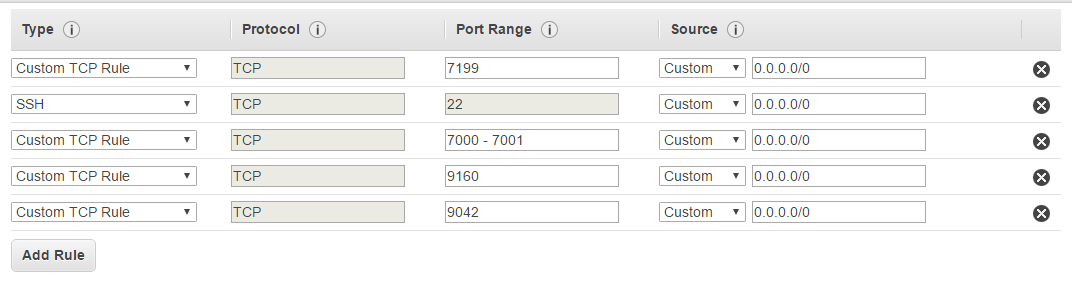
\includegraphics[width=\linewidth]{images/inbound-rules-cassandra.PNG}
  		\caption{security settings.}
  		\label{fig:security-settings}
	\end{figure}
	
	\par
	Indien deze stap afgehandeld is, krijgen we een overzicht te zien. 
	Als alles naar wens is klikken we op ‘Launch’ waardoor er een prompt opengaat. 
	Vanuit deze prompt kunnen we een pem-file aanmaken en downloaden, het is zeer belangrijk om 
	deze op een veilige plaats op te slaan, deze nodig is om via ssh een connectie naar onze machines te maken. 
	Bij het aanmaken van nieuwe machines kunnen we dezelfde pem-file hergebruiken zodat we één key hebben voor al onze instances.
	 We slagen het bestand op onder aem-ec2.pem.
	
	\subsubsection{Cassandra als service}
	Nu we onze machines hebben is het tijd om hiervan Cassandra nodes te maken. 
	Via het ‘Instance’ scherm kunnen we achterhalen wat de publieke IP-adressen zijn van deze machines 
	(laten we ervan uitgaan dat deze 1.0.0.1,1.0.0.2 en 1.0.0.3 zijn.). 
	Volgende stap moet op elke machine identiek herhaalt worden buiten de nodige aanpassingen aan de cassandra.yaml. 
	Laten we eerst op onze machines inloggen via het commando:
	
	\begin{lstlisting}
		$ ssh –i aem-ec2.pem ec2-user@1.0.0.1 
	\end{lstlisting}
	
	Nu zijn we ingelogd als ec2-user op onze machine. Om Cassandra 3.x te kunnen draaien hebben we Java 1.8 nodig, 
	via het commando ‘java -version’ kunnen we dit controleren. 
	Indien de versie lager ligt, zijn we verplicht om Java 1.8 te installeren. Een mogelijke manier om dit te doen is als volgt:	
	\par
	We navigeren naar onze jvm folder
	\begin{lstlisting}
  		$ cd /usr/lib/jvm
	\end{lstlisting}
	\par
	Vervolgens downloaden we de java 1.8 tar file
	\begin{lstlisting}
		$ sudo wget --no-cookies --no-check-certificate --header "Cookie: gpw_e24=http://www.oracle.com/; oraclelicense=accept-securebackup-cookie" http://download.oracle.com/otn-pub/java/jdk/8u121-b13/e9e7ea248e2c4826b92b3f075a80e441/jdk-8u121-linux-x64.tar.gz
	\end{lstlisting}
	
	\par
	En pakken we deze uit
	\begin{lstlisting}
		$ sudo tar xzf jdk-8u121-linux-x64.tar.gz
	\end{lstlisting}
	
	\par
	Na het uitpakken kunnen we onze jdk registreren als java optie
	\begin{lstlisting}
		$ sudo alternatives --install /usr/bin/java java /usr/lib/jvm/jdk1.8.0_121/bin/java 2
	\end{lstlisting}
	
	\par
	Als we nu het volgende commando runnen zien we twee java mogelijke java engines, diegene dat al geïnstalleerd was en onze nieuwe. 
	Hier kiezen we om onze nieuwe als default te gebruiken.
	\begin{lstlisting}
		$ sudo alternatives --config java
	\end{lstlisting}
	\begin{lstlisting}
		$ Enter to keep the current selection[+], or type selection number: 2
	\end{lstlisting}
	
	\par
	Als alles correct verlopen is zien we nu 1.8 staan wanneer we opnieuw het commando ‘java -version’ uitvoeren.
	
	\par
	Nu volgt de installatie van Cassandra zelf, hierbij is de eerste stap het toevoegen van de datastax.repo zodat we via het yum commando Cassandra kunnen installeren.
	 Als dit gebeurt is kunnen we via yum zowel Cassandra als Nodetool installeren.
	\par
	Maak het bestand datastax.repo aan.
	\begin{lstlisting}
		$ sudo touch /etc/yum.repos.d/datastax.repo
	\end{lstlisting}
	
	\par
	Maak het bestand datastax.repo aan.
	\begin{lstlisting}
		$ sudo touch /etc/yum.repos.d/datastax.repo
	\end{lstlisting}
	
	\par
	Vul deze met de nodige data
	\begin{lstlisting}
		$ sudo touch /etc/yum.repos.d/datastax.repo
	\end{lstlisting}
	En zorg dat deze conform is aan Figuur \ref{fig:datastax.repo}
	\begin{figure}[h!]
  		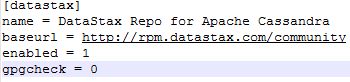
\includegraphics[width=\linewidth]{images/datastax-repo.PNG}
  		\caption{datastax.repo}
  		\label{fig:datastax.repo}
	\end{figure}
	
	\par
	Nu kunnen we Cassandra en Nodetool installeren.
	\begin{lstlisting}
		$ sudo yum install dsc30
	\end{lstlisting}
	\begin{lstlisting}
		$ sudo yum install cassandra30-tools
	\end{lstlisting}
	
	\par
	Als we nu Cassandra zouden opstarten op de 3 machines, hebben we 3 clusters met elks 1 node gemaakt. 
	Vanzelfsprekend is dit niet het gezochte resultaat en willen we 1 cluster met 3 nodes, om dit mogelijk te maken moeten we de aanpassingen maken, getoond in Figuur \ref{fig:cassandra.yaml} (locatie: /etc/cassandra/conf/cassandra.yaml).
	\begin{figure}[h!]
  		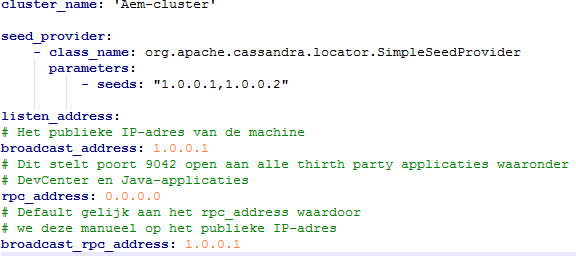
\includegraphics[width=\linewidth]{images/cassandra-yaml.PNG}
  		\caption{cassandra.yaml}
  		\label{fig:cassandra.yaml}
	\end{figure}
	
	\par
	Nu dat onze yamls correct staan kunnen we op onze machines cassandra starten met het commando ‘sudo service cassandra start’. 
	Na enkele minuten zien we dan dat de 3 nodes elkaar gevonden hebben via het commando ‘nodetool status’.
	
	\par
	\subsubsection{DevCenter}
	 Nu we onze databank hebben kunnen we onze nodige modellen toevoegen, het gebruikte script kan je terugvinden in de bijlagen.
	 Voor het uitvoeren van deze scripts kan gebruikt maken van DevCenter, een open-source tool waarmee een connectie kan gemaakt worden met een cluster. 
	 Deze manier van werken is aangenamer dan telkens te moeten sshen naar een node om daar via het cqlsh commando onze databank te kunnen querieën. 
	 Onze drie tabellen die we gaan gebruiken zijn Product, Category en Price. 
	 Deze drie vertonen elk een andere graad van dynamiek, gepast voor het onderzoek dat we zullen verrichten.
	 We voorzien telkens ook een log tabel voor deze drie zodat we aan de hand van een datum, die fungeert als ondergrends, de gewijzigde rijen kunnen opvragen.
	 Eenmaal onze databank operationeel is kunnen we beginnen aan de service die deze zal aanspreken.
\end{document}